\subsection{実験設定}
\subsubsection{データセット}
CVC-ClinicDBデータセット\cite{BERNAL201599}データセットおよびKvasir-SEGデータセット\cite{jha2020kvasir}を用いて実験を行った.
CVC-ClinicDBデータセットは$612$枚の大腸内視鏡画像($384 \times 288$ pixel),Kvasir-SEGデータセットは$1000$枚の大腸内視鏡画像で,
いずれも大腸内視鏡画像とそれに対応するポリープの正解マスクから構成される.
データは$5$分割交差検証で分割され,CVC-ClinicDBデータセットに関しては同一のビデオシーケンスが異なるfoldに跨がらないよう,GroupKFoldを用いた分割を行った.

\subsubsection{実装の詳細}
セグメンテーションモデルにはTable~\ref{tab:unet_architecture}に示される構造のU-Net\cite{ronneberger2015u}を採用した.
学習にはAdam optimizer\cite{kingma2014adam}を使用し,バッチサイズ$32$, 学習率$10 ^ {-3}$に設定した.
前処理として全画像を$W = 224$ pixel, $H = 224$ pixelにリサイズし,訓練時には
$50\%$の確率で上下左右反転および明度・コントラストの変更を適用した.
最大エポック数$E$は$200$に設定した.

MC Dropoutによる不確実評価は,$\tau=10$エポックごとに実施した.
Dropout層はエンコーダの最終ブロックとデコーダの最終ブロックに配置し,
各評価時には,先行研究\cite{pmlr-v48-gal16}を基に$p = 0.5$で$T = 10$回の確率的推論を行った.
またデータセット内の難易度指標の正規化時のパーセンタイルは難易度分布の偏りを考慮して$q = 25$に設定し,
予備実験の結果を基に適応的学習の開始エポックは$E_0 = 10$とし,
$\epsilon_{\text{min}}=0$, $\epsilon_{\text{max}}=0.5$, $k=2$とした.


\subsubsection{比較条件}
適応的学習の有効性を評価するため,以下の手法と提案法を比較する:

\begin{itemize}
    \item Dice Loss\cite{milletari2016v}:医用画像セグメンテーションにおける標準的な損失関数であり,ベースラインとして採用した.
    \item Focal Loss\cite{lin2017focal}:易しいサンプルの損失を down-weight することで
    クラス不均衡に対処する手法であり,
    提案法と「サンプルの難易度に応じた重み付け」という点で動機が共通する.
    ただし,Focal Loss は予測確信度に基づく静的な重み付けであるのに対し,
    提案法はモデルの不確実性に基づく動的な重み付けである点が異なる.
    また易しいサンプルの損失を down-weight する割合は$\gamma = 2$とした.
    \item PolyDice-1 Loss ($\epsilon = 0$):PolyDice-1 Loss の標準形式であり,
    理論上は通常の Dice Lossを近似したものである.
    提案法および後述する Optimal 設定との比較において,
    パラメータ $\epsilon$ を操作すること自体の純粋な効果を検証するための基準として採用した.
    \item PolyDice-1 Loss (optimal):固定$\epsilon$による性能の理論的上界を評価するため,
    テストデータに対する Dice 係数を最大化する$\epsilon$値を事後的に探索し,
    これを理想設定として比較に含めた.具体的には,
    $\epsilon \in \{-0.3, -0.2, \ldots, 0.5\}$ の範囲で網羅的に評価し,
    最高精度を達成する値$\epsilon$をデータセットごとに決定した.
    この設定は実運用では実現不可能であるが,
    「最適な固定値が事前に既知である」という理想的な条件下での性能を表す.
\end{itemize}

これらの比較により,(1) 提案法が標準的な損失関数より優れているか,
(2) 適応的$\epsilon$制御が固定$\epsilon = 0$より有効か,(3) 提案法が Optimal 設定に匹敵あるいは上回る性能を達成できるか,を検証する.

\subsubsection{評価指標}

またセグメンテーションの性能の評価には,領域の重なりを測るDice係数およびIoU(Intersection over Union)および検出精度を測るPrecisionおよびRecallを用いた.
画像$n$に対するモデルの予測マップ $$\hat{\mathbf{Y}}_n$$に対し,閾値 $\theta_\text{th} = 0.5$ で二値化した予測マスク $\tilde{Y}_n = \{\tilde{y}_{n,i,j}\}$ とする.
画像$n$に対する真陽性 (TP),偽陽性 (FP),偽陰性 (FN) の画素数はそれぞれ以下で定義される.

\begin{align}
    TP_n &= \sum_{j=1}^{W} \sum_{i=1}^{H} \tilde{y}_{i, j} y_{i, j} \\
    FP_n &= \sum_{j=1}^{W} \sum_{i=1}^{H} \tilde{y}_{i, j} (1 - y_{i, j}) \\
    FN_n &= \sum_{j=1}^{W} \sum_{i=1}^{H} (1 - \tilde{y}_{i, j}) y_{i, j}
\end{align}

\begin{itemize}
    \item Dice係数: 正解領域と予測領域の重複度を直接評価するもので,医用画像のような不均衡な画像でも,微小な対象物の抽出精度を適切に反映できるため,主指標として採用した.
    \begin{align}
        \text{Dice}_n = \frac{2TP_n}{2TP_n + FP_n + FN_n}
        % &= \frac{2TP}{2TP + FP + FN}
    \end{align}

    \item IoU:予測領域と正解領域の共通部分を評価する指標であり,セグメンテーションタスクにおける一般的な評価指標として広く用いられている.
    \begin{align}
        \text{IoU}_n = \frac{TP_n}{TP_n + FP_n + FN_n}
    \end{align}

    \item Precision:モデルが抽出した領域の正解率を評価する指標であり,過剰な検出を抑制する性能を定量化するために採用した.
    \begin{align}
        \text{Precision}_n = \frac{TP_n}{TP_n + FP_n}
    \end{align}

    \item Recall:正解領域をどの程度検出できているかを評価する指標であり,特に病変の見落としを防ぐ性能を検証するために採用した.
    \begin{align}
        \text{Recall}_n = \frac{TP_n}{TP_n + FN_n}
    \end{align}
\end{itemize}

各指標はテストデータ全体での平均値を報告する.

\clearpage

\begin{table}[t]
    \centering
    \caption{Architecture of the U-Net model used in experiments. Each layer shows the output spatial resolution and number of channels.}
    \label{tab:unet_architecture}
    \begin{tabular}{lc}
        \toprule
        \textbf{Layer} & \textbf{Output Size} \\
        \midrule
        % ★★★ 表示するテキストを追加 ★★★
        \multicolumn{2}{c}{\textit{--- Encoder ---}} \\
        Input & $224 \times 224 \times 3$ \\
        inc (DoubleConv) & $224 \times 224 \times 64$\\
        down1 (MaxPool + DoubleConv) & $112 \times 112 \times 128$ \\
        down2 (MaxPool + DoubleConv) & $56 \times 56 \times 256$ \\
        down3 (MaxPool + DoubleConv) & $28 \times 28 \times 512$ \\
        down4 (MaxPool + DoubleConv) & $14 \times 14 \times 512$ \\
        \midrule
        % ★★★ 表示するテキストを追加 ★★★
        \multicolumn{2}{c}{\textit{--- Decoder ---}} \\
        up1 (Upsample + DoubleConv) & $28 \times 28 \times 256$ \\
        up2 (Upsample + DoubleConv) & $56 \times 56 \times 128$ \\
        up3 (Upsample + DoubleConv) & $112 \times 112 \times 64$ \\
        up4 (Upsample + DoubleConv) & $224 \times 224 \times 64$ \\
        \midrule
        outc (Conv2d) & $224 \times 224 \times 2$ \\
        \bottomrule
    \end{tabular}
\end{table}

\clearpage

\subsection{結果と議論}

\subsubsection{比較手法との性能比較}
Table~\ref{tab:benchmark_cvc_clinicdb} および Table~\ref{tab:benchmark_kvasir_seg} に,各データセットにおける比較手法との性能比較を示す.両データセットにおいて,
提案法は全ての比較手法を上回る性能を達成した.Focal Loss は両データセットにおいて Dice Loss を下回る結果となった.
特に注目すべきは,テストデータに対して最適な固定$\epsilon$を事後探索したPolyDice-1 Loss (optimal) をも上回った点である(Fig. \ref{fig:epsilon_comparison}).
固定$\epsilon$では全画像に同一の勾配特性が適用されるため,
容易な画像への過学習と困難な画像の学習不足が同時に生じうる.さらに,学習進行に伴い各画像の相対的な難易度は変化するが,
固定 $\epsilon$ ではこの変化に追従できない.提案法は$\tau$エポックごとに難易度を再評価し,$\epsilon$を動的に更新することで,これらの問題を回避している.

なお,Focal Loss は容易なサンプルの損失を低減することでクラス不均衡に対処する手法であるが,セグメンテーションタスクでは画像単位ではなくピクセル単位で生じる.
そのため,ピクセルの予測不確実性のみに基づく重み付では,画像全体としてのセグメンテーション難易度を適切に反映できなかったと考えられる.

\subsubsection{難易度別の性能分析}
提案手法の設計意図である「困難な症例に対しては急峻な勾配を与え,容易な症例に対しては
緩やかな勾配を与える」という適応的学習戦略の有効性を検証するため,
症例の難易度に基づいた層別分析を行った.難易度の分類には,提案法とは独立した基準として,ベースラインであるDice Lossで学習したモデルの
テストデータに対するDice 係数を用いた.具体的には,Dice係数が
下位$33$パーセンタイル未満の症例を「困難(Hard)」,$33$パーセンタイル以上$66$パーセンタイル未満を「中程度(Medium)」,
$66$パーセンタイル以上を「容易(Easy)」と定義した.

Fig. \ref{fig:difficulty_comparison} に,両データセットにおける各難易度層別の性能比較を示す.Hard群において,提案法はベースラインであるDice Loss と比較してDice 係数が CVC-ClinicDB で$0.32$,
Kvasir-SEG で$0.13$向上した. これは,不確実性が高く困難と判定された症例に対して大きな $\epsilon$ を割り当て,
損失関数の勾配を急峻にしたことで,モデルがこれらの画像の特徴を重点的に学習できたことを示唆している.
一方,EasyおよびMedium群においては,精度変化が小さく一部でわずかな低下も見られた.この結果は,
十分に学習が進んだ症例からの勾配を相対的に抑制するという設計意図を反映しており,
容易なパターンへの過学習を防いだ結果と解釈できる.以上の結果から,提案法による全体性能の向上は,主として困難な症例における大幅な改善に起因することが確認された.

\subsubsection{適応的制御のメカニズム分析}
提案手法の動作メカニズムを理解するため,訓練データに対するパラメータ $\epsilon$ の推移を難易度別に分析した.
Fig. \ref{fig:epsilon_evolution}に,CVC-ClinicDBデータセットにおける各難易度層別の$\epsilon$の推移を示す.
分析の結果,各群の$\epsilon$の分布には明確な分離が見られなかった.
特に注目すべきは学習初期($10 \text{--} 40$エポック付近)の挙動であり,最終的にEasyと分類される画像群の $\epsilon$ が,Hard群よりも高い値を示す傾向が観察された.

この一見矛盾する結果は,難易度分類と$\epsilon$算出の基準の違いに起因すると解釈できる.
本研究における難易度分類は,Dice Lossを用いたベースラインモデルの学習完了後の最終精度に基づく事後的な指標である.
一方,$\epsilon$ は各時点におけるモデルの不確実性から動的に算出される.この定義の乖離が学習段階に応じて各群の$\epsilon$が異なる挙動を示したと考えられる.

具体的には,学習初期においてEasy群の画像はモデルにとって未学習の状態であるため,予測のばらつきが大きく,算出される不確実性が一時的に高くなる.
一方,Hard群の画像に対しては,モデルがその複雑さを認識できるほどの特徴抽出能力をまだ獲得しておらず,誤った領域を高い確信度で予測する過信(Overconfidence)が生じる.
その結果,Hard群に対する不確実性が過小評価され,$\epsilon$ が相対的に低く抑えられたと考えられる.
学習の進行に伴い,Easy群は,速やかに安定した特徴表現を獲得し,予測のばらつきが収束するため,$\epsilon$ は急速に低下する.
これに対し,Hard群ではモデルが徐々に症例の複雑さを認識し始め,不確実性が適切に上昇することで$\epsilon$の値が上昇に転じる.

以上の分析から,提案法が静的な難易度ラベルに基づく重み付けではなく,モデルの現在の学習状態に応じた動的な勾配調整として機能していることが示唆される.
すなわち,「困難な画像に大きな勾配を与える」というよりも,「既に学習が完了した画像の勾配を抑制し,未学習の画像への学習を促進する」メカニズムとして解釈できる.
この動的な適応制御が,結果として困難な症例の学習促進に寄与していると考えられる.

続いて,$\epsilon$の動的制御が学習過程に与える影響を検証するため,訓練データに対するDice係数の推移を難易度群別に分析した.
Fig. \ref{fig:convergence_ci99}に結果を示す.Easy群およびMedium群では,提案法とベースラインの間に顕著な差は見られず,両手法ともに学習初期から急速に高精度へ収束した.
一方,Hard群では提案法がベースラインを一貫して上回り,学習後期においてその差がさらに拡大する傾向が観察された.

この結果は,Fig. \ref{fig:epsilon_evolution}で示した$\epsilon$の推移と整合的である.学習初期においてEasy群の$\epsilon$が一時的に高くなることで学習が促進され,その後$\epsilon$が低下することで過学習が抑制される.
一方,Hard群では$\epsilon$が学習の進行とともに上昇し,継続的な学習信号の強化が行われる.この動的な勾配調整により,結果として困難な症例の学習が促進されたと考えられる.

\clearpage

\begin{figure}[t]
    \centering
    \includegraphics[width=\linewidth]{figure/fig_epsilon_comparison.pdf}
    \caption{Comparison of segmentation performance (Dice coefficient) between the proposed adaptive method and PolyDice-1 Loss with various fixed $\epsilon$ values. The left graph shows the results for the CVC-ClinicDB dataset, and the right graph shows the results for the Kvasir-SEG dataset. The red dashed line represents the performance of the proposed method, demonstrating robustness comparable to or exceeding the optimal fixed parameter settings.}
    \label{fig:epsilon_comparison}
\end{figure}

\clearpage

\begin{table}[t]
    \centering
    \caption{Performance Comparison with Existing Loss Functions on CVC-ClinicDB Dataset}
    \label{tab:benchmark_cvc_clinicdb}
    \begin{tabular}{ccccc} % lcccc から ccccc に変更(全て中央揃え)
        \toprule
        Method & Dice & IoU & Precision & Recall \\ % Dice Coefficient -> Dice に短縮
        \midrule
        Dice Loss & 0.5408 & 0.4347 & 0.6359 & 0.5819 \\
        Focal Loss ($\gamma = 2$) & 0.5007 & 0.4133 & 0.7078 & 0.4707 \\
        PolyDice-1 ($\epsilon=0$) & 0.5825 & 0.4808 & 0.6817 & 0.6167 \\ % fixed, .0 を削除
        PolyDice-1 (Opt. $\epsilon$) & 0.6145 & 0.5145 & 0.7090 & 0.6372 \\ % optimized, fixed を短縮
        \midrule
        Adaptive PolyDice-1 & \textbf{0.6924} & \textbf{0.5262} & \textbf{0.7827} & \textbf{0.7113} \\
    \bottomrule
    \end{tabular}
\end{table}

\begin{table}[t]
    \centering
    \caption{Performance Comparison with Existing Loss Functions on Kvasir-SEG Dataset}
    \label{tab:benchmark_kvasir_seg}
    \begin{tabular}{ccccc} % lcccc から ccccc に変更(全て中央揃え)
        \toprule
        Method & Dice & IoU & Precision & Recall \\ % Dice Coefficient -> Dice に短縮
        \midrule
        Dice Loss & 0.7895 & 0.7021 & 0.8281 & 0.8154 \\
        Focal Loss ($\gamma = 2$) & 0.7192 & 0.6082 & 0.8634 & 0.6769 \\
        PolyDice-1 ($\epsilon=0$) & 0.8095 & 0.7198 & 0.8461 & 0.8268 \\ % fixed, .0 を削除
        PolyDice-1 (Opt. $\epsilon$) & 0.8095 & 0.7198 & 0.8461 & 0.8268 \\ % optimized, fixed を短縮
        \midrule
        Adaptive PolyDice-1 & \textbf{0.8272} & \textbf{0.7440} & \textbf{0.8707} & \textbf{0.8397} \\
    \bottomrule
    \end{tabular}
\end{table}

\clearpage

\begin{figure}[t]
    \centering
    \includegraphics[width=\linewidth]{figure/fig_difficulty_comparison.pdf}
    \caption{Stratified performance comparison of the Dice coefficient across three difficulty levels (Easy, Medium, Hard) on the CVC-ClinicDB (left) and Kvasir-SEG (right) datasets. The proposed Adaptive PolyDice-1 Loss (red bars) demonstrates consistent improvements over the baseline Dice Loss (blue bars), particularly in the ``Hard'' category, where significant performance gains ($+0.32$ and $+0.13$) are observed.}
    \label{fig:difficulty_comparison}
\end{figure}

\clearpage

\begin{figure}[t]
    \centering
    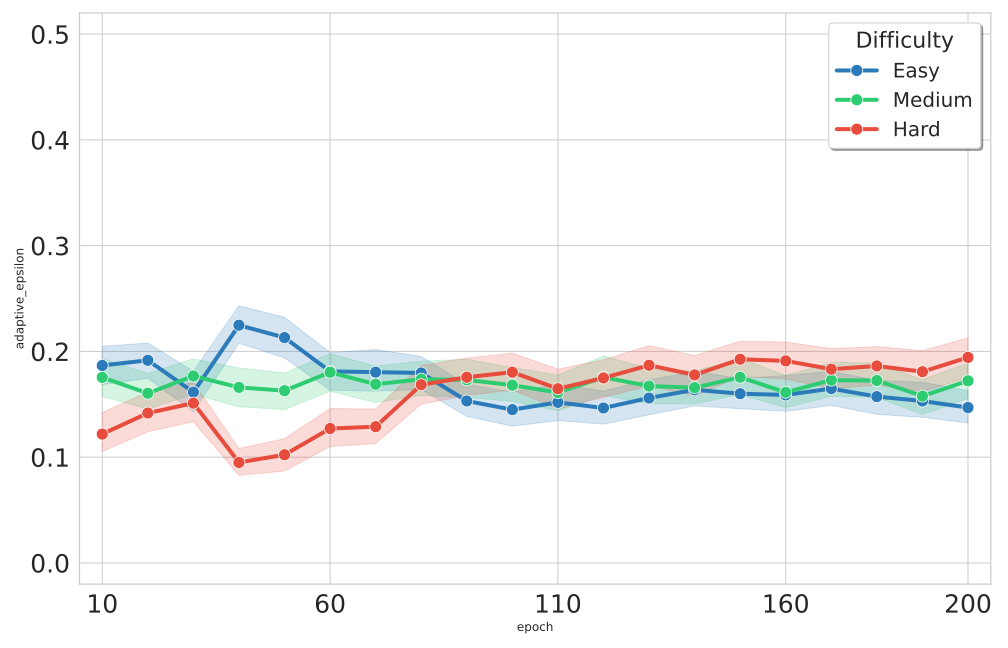
\includegraphics[width=\linewidth]{figure/epsilon_combined_lineplot_ci.pdf}
    \caption{Evolution of the adaptive parameter $\epsilon$ throughout the training process on the CVC-ClinicDB dataset. Cases are categorized into ``Easy,'' ``Medium,'' and ``Hard'' based on their baseline segmentation performance. Solid lines represent the mean values, and shaded regions denote the $99\%$ confidence intervals.}
    \label{fig:epsilon_evolution}
\end{figure}

\clearpage

\begin{figure}[t]
    \centering
    \includegraphics[width=\linewidth]{figure/difficulty_lineplot_comparison_ci99.pdf}
    \caption{Dice coefficient transitions throughout training for different difficulty levels on CVC-ClinicDB. Curves show the mean values of the proposed (red) and baseline (gray) methods, with shaded areas indicating 99\% confidence intervals.}
    \label{fig:convergence_ci99}
\end{figure}

\clearpage

\subsubsection{ハイパーパラメータの影響}
本節では,提案法における主要なハイパーパラメータの感度分析を行い,設計選択の妥当性を検証する.

\textbf{$\epsilon$ 範囲の影響:}
Table~\ref{tab:ablation_epsilon_cvc}およびTable~\ref{tab:ablation_epsilon_kvasir-seg}に示すように,
$\epsilon$ の変動範囲を $[0, 0.5]$ と設定した場合に,両データセットにおいて最も良好なセグメンテーション性能が得られた.
上限値$\epsilon_{\text{max}}$を $0.3$ から $0.5$ へ拡大したことで,
困難な症例に対してより大きな $\epsilon$ を割り当て可能となり,損失関数の勾配が適切に強調され,病変特徴の学習が促進されたと考えられる.
一方,下限値$\epsilon_{\text{min}}$を $-0.3$ まで拡張した設定
($\epsilon_{\text{min}}=-0.3, \epsilon_{\text{max}}=0.5$)では,$\epsilon_{\text{min}}=0$ の場合と比較して性能が向上しなかった.
これは,変動範囲の過度な拡大により不確実性推定に含まれる微細なノイズに対する感度が必要以上に高まり,
学習の安定性を損なったためと考えられる.

\textbf{感度パラメータ$k$の影響:}
Table~\ref{tab:ablation_k_cvc}およびTable~~\ref{tab:ablation_k_kvasir-seg}に,難易度スコアに対するシグモイド関数の傾き $k$ を変化させた結果を示す.
Kvasir-SEG データセットでは $k=2$ の場合に最も精度が高く,CVC-ClinicDBでは$k=3$がわずかに高い値を示したものの, $k=2$も同等の性能を達成した.
$k=1$ のように傾きが緩やかすぎる場合,難易度の差が損失形状に十分に反映されない.逆に $k=3$ のように急峻すぎる場合,損失形状が二値的に切り替わり,学習が不安定になる可能性がある.
以上より,$k=2$ が難易度に応じた滑らかな適応と安定した学習の両立において適切な設定であると考えられる.

\textbf{適応開始エポック$E_0$の影響:}
Fig. \ref{fig:ablation_e0}に示すように,適応的学習の開始タイミングは早いほど良好な結果をもたらし,
最も早い$E_0 = 10$において最高性能を記録した.4.2.3で示したように,学習初期の段階で既に症例間の学習進度に明確な差異が生じており(Fig. \ref{fig:convergence_ci99}参照),
この段階から適応的制御を開始することで,未学習の症例への学習促進効果を最大化できたと考えられる.

\clearpage

\begin{table}[t]
    \centering
    \caption{Impact of the adaptive $\epsilon$ range $[\epsilon_{\text{min}}, \epsilon_{\text{max}}]$ on segmentation performance (CVC-ClinicDB dataset).}
    \label{tab:ablation_epsilon_cvc}
    \begin{tabular}{cccccc}
        \toprule
        $\epsilon_{\text{min}}$ & $\epsilon_{\text{max}}$ & Dice & IoU & Precision & Recall \\
        \midrule
        $0$ & $0.3$ & \textbf{0.7017} & \textbf{0.6050} & \textbf{0.7875} & \textbf{0.7234} \\
        $0$ & $0.5$ & 0.6924 & 0.5913 & 0.7827 & 0.7113 \\
        $-0.3$ & $0.5$ & 0.7000 & 0.5993 & 0.7818 & 0.7220 \\
        \bottomrule
    \end{tabular}
\end{table}

\begin{table}[t]
    \centering
    \caption{Impact of the adaptive $\epsilon$ range $[\epsilon_{\text{min}}, \epsilon_{\text{max}}]$ on segmentation performance (Kvasir-SEG dataset).}
    \label{tab:ablation_epsilon_kvasir-seg}
    \begin{tabular}{cccccc}
        \toprule
        $\epsilon_{\text{min}}$ & $\epsilon_{\text{max}}$ & Dice & IoU & Precision & Recall \\
        \midrule
        $0$ & $0.3$ & 0.8239 & 0.7391 & 0.8608 & 0.8410 \\
        $0$ & $0.5$ & \textbf{0.8272} & \textbf{0.7440} & \textbf{0.8707} & 0.8397 \\
        $-0.3$ & $0.5$ & 0.8189 & 0.7313 & 0.8537 & \textbf{0.8454} \\
        \bottomrule
    \end{tabular}
\end{table}

\begin{table}[t]
    \centering
    \caption{Sensitivity analysis of the sigmoid slope parameter $k$ in the control function (CVC-ClinicDB dataset).}
    \label{tab:ablation_k_cvc}
    \begin{tabular}{ccccc}
        \toprule
        $k$ & Dice & IoU & Precision & Recall \\
        \midrule
        $1$ & 0.6935 & 0.5962 & 0.7853 & 0.7175 \\
        $2$ & 0.6924 & 0.5913 & 0.7827 & 0.7113 \\
        $3$ & \textbf{0.7063} & \textbf{0.6084} & \textbf{0.8010} & \textbf{0.7178} \\
        \bottomrule
    \end{tabular}
\end{table}

\begin{table}[t]
    \centering
    \caption{Sensitivity analysis of the sigmoid slope parameter $k$ in the control function (Kvasir-SEG dataset).}
    \label{tab:ablation_k_kvasir-seg}
    \begin{tabular}{ccccc}
        \toprule
        $k$ & Dice & IoU & Precision & Recall \\
        \midrule
        $1$ & 0.8235 & 0.7404 & 0.8589 & \textbf{0.8440} \\
        $2$ & \textbf{0.8272} & \textbf{0.7440} & \textbf{0.8707} & 0.8397 \\
        $3$ & 0.8229 & 0.7375 & 0.8663 & 0.8370 \\
        \bottomrule
    \end{tabular}
\end{table}

\begin{figure}
    \centering
    \includegraphics[width=\linewidth]{figure/fig_E0_effect.pdf}
    \caption{Effect of adaptation start epoch $E_0$ on segmentation performance (Dice coefficient) for the CVC-ClinicDB (left) and Kvasir-SEG (right) datasets. }
    \label{fig:ablation_e0}
\end{figure}

\clearpage
\subsubsection{定性的評価}
Fig. \ref{compare} に,CVC-ClinicDB データセットにおける各難易度層の代表的な症例について,比較手法と提案法のセグメンテーション結果を示す.
境界が明瞭な容易な症例および中程度の症例においては,既存手法と提案法の両方が高精度なセグメンテーションを実現している.
一方,ポリープと粘膜壁のコントラストが低く境界が不明瞭な困難な症例において,
ベースラインであるDice Loss やFocal Loss ではポリープ領域を捉えきれず,著しい過少検出が発生した.
PolyDice-1 Loss (optimal) においても検出が不完全である.
これに対し,提案法はポリープ境界を適切に捉えており,良好なセグメンテーション結果を達成している.
この結果は,提案法がMC Dropout により当該症例を困難な画像と判定し,
損失関数の形状パラメータ$\epsilon$を大きく設定したことで,
学習時に勾配が強化され,低コントラスト領域における特徴抽出能力が向上したことを示唆している.
\clearpage

\begin{figure*}[t]
    \centering % 図を中央揃えにする(推奨)
    \includegraphics[width=\linewidth]{figure/compare.pdf}
    \caption{Qualitative comparison of segmentation results on the CVC-ClinicDB dataset. Each row represents a different difficulty level (easy, medium, hard), categorized by baseline Dice Loss performance.}
    \label{compare}
\end{figure*}